\head{Олимпиадное программирование}
В данном разделе мы получим некоторое представление об олимпиадном программировании, а именно, узнаем, как выглядит олимпиадная задача, и что такое \term{сложность алгоритмов}.

\subhead{Олимпиадная задача}
Посмотрим на пример того, как выглядит олимпиадная задача:

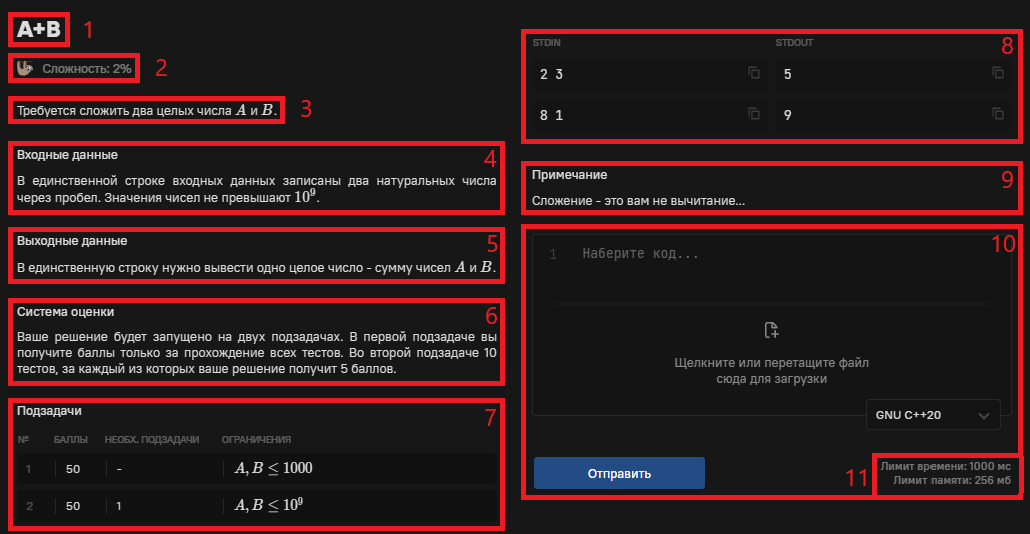
\includegraphics[scale=0.66]{img/task.png}

Теперь разберёмся со всеми её частями:
\begin{enumerate}
    \item Название задачи.
    \item Сложность — на олимпиадах такого пункта нет, также сложность есть не на всех сайтах для олимпиадного программирования.
    \item Условие задачи — здесь может быть какое-то введение к задаче или список действий, которые должна выполнять программа. 
    \item В описание входных данных написано, как программе вводятся данные.
    \item В описание выходных данных написано, как выводить ответы к задаче.
    \item Блок с системой оценивания может отсутствовать, но если он есть, то в нём описывается, как начисляются баллы за задачу.
    \item Блок с подзадачами тоже может отсутствовать (вместе с системой оценивания).
    \item Примеры того, какие ответы программа должна выводить при каких входных данных. Баллы за примеры обычно не ставятся.
    \item В примечании может быть описано, как получились именно такие ответы для примеров.
    \item Собственно, поле для отправки Вашей программы.
    \item Ограничения по времени и памяти (об этом ещё будет чуть дальше).
\end{enumerate}

Когда Вы участвуете в какой-либо олимпиаде, тот там предоставляется несколько задач. При этом за каждую задачу можно получить максимум 100 баллов (обычно), и цель — набрать как можно больше баллов. Также запоминается время, за которая были решены задачи, и если у людей равенство по баллам, то они могут сортироваться по времени (чем меньше суммарное время, тем лучше). Отношение к ошибочным посылкам у олимпиад может быть разным: где-то их количество не имеет значение, но где-то за каждую не правильную посылку даётся штрафное время.

За каждое отправленное решение можно получить один из следующих вердиктов:
\begin{itemize}
    \item \textcolor{dark_green}{Accept} — правильное решение.
    \item \textcolor{red}{WA (\term{Wrong Answer})} — неверный ответ на одном из тестов.
    \item \textcolor{red}{TLE (\term{Time limit exceeded})} — превышено ограничение по времени.
    \item \textcolor{red}{MLE (\term{Memory limit exceeded})} — превышено ограничение по памяти.
    \item \textcolor{red}{Error} — также могут быть какие-либо другие ошибки: ошибка компиляции, неправильный формат вывода, ошибка во время выполнения и т.д.
\end{itemize}

\subhead{Сложность алгоритма}
Основным критерием качества алгоритма является его сложность. Как можно понять по ограничениям, различают сложности по памяти и времени.

Сложность алгоритма по памяти оценивается довольно просто: складываются размеры всех используемых переменных. Если какая-то переменная является контейнером и хранит в себе другие переменные, то, логично, её размер определяется как сумма размеров всех хранимых элементов. С размерами разных переменных мы ознакомимся чуть позже, а пока перейдём к временной сложности алгоритмов.

Временная сложность оценивает, как долго будет выполняться алгоритм. А зная это, мы уже можем понять, пройдёт ли решение ограничение по времени. Обозначается сложность буквой $O$ при этом буквой $n$ часто обозначают размер входных данных. Например, сложность может быть $O(n)$.

Если в алгоритме используются циклы, то сложность оценивается по количеству его итераций; если циклы вложены, то количество их итераций перемножается; если же циклы идут последовательно, то сложность определяется суммой сделанных итераций.

При этом, поскольку нужно только оценить сложность алгоритма, то все константы опускаются, и оставляется только наибольшая степень. Например, если в алгоритме есть последовательные циклы со количеством итераций $100$, $2n$ и $0.5n^2$, то сложность будет $O(100 + 2n + 0.5n^2) = O(1 + n + n^2) = O(n^2)$. Более формальное определение таково: если сложность алгоритма составляет $O(x)$, то это значит, что начиная с какого-то размера входных данных ($n_0$) алгоритм совершает не более, чем $c \cdot x$ операций. Согласно такому определения, можно говорить, что сложность алгоритма с $n$ итерациями, это $O(n^2)$, но так делать не принято и стараются оценивать сложность точнее.

Также, иногда применяются другие оценки сложности: $\Omega(x)$ — \term{нижняя граница} и $\Theta(x)$ — \term{точная граница}. Нижняя граница говорит, что алгоритм начиная с какого-то $n_0$ совершает не менее $c \cdot x$ операций, а точная граница говорит, точное число операций, и, как следствие, должно выполняться равенство $\Theta(x) = \Omega(x) = O(x)$. Но мы будем использовать только $O$-нотацию.

Как только мы оценили количество выполняемых операций, то можем легко узнать, как долго будет выполняться алгоритм, ведь компьютер умеет выполнять примерно $2 \cdot 10^7 \dash 2 \cdot 10^8$ операций в секунду.
